\section{Auswertung}
\begin{figure}
    \centering
    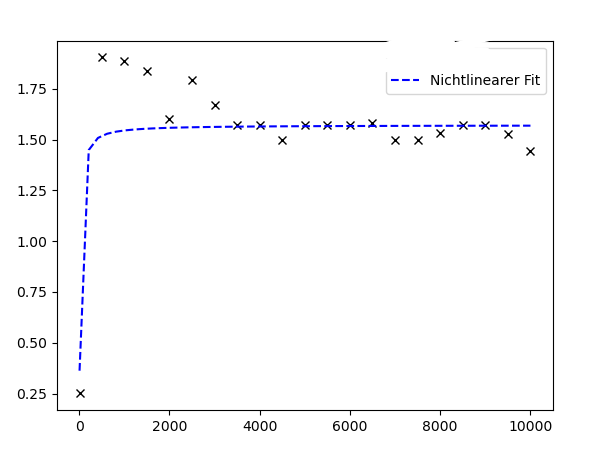
\includegraphics[width=0.6\textwidth]{build/plot1.pdf}
    \caption{Schematischer Aufbau des Lock-In-Verstäker mit installiertem Photodetektor. \cite{skript}} 
    \label{fig:licht}
\end{figure}

\begin{figure}
    \centering
    \includegraphics[width=0.6\textwidth]{build/plot2.pdf}
    \caption{Schematischer Aufbau des Lock-In-Verstäker mit installiertem Photodetektor. \cite{skript}} 
    \label{fig:licht2}
\end{figure}
Untersucht wurden die Ausgangsspannungen am Lock-In-Verstäker in Abhängigkeit von dem Phasenunterschied zwischen Signal- und Referenzspannung. Im Folgenden ist die Auswertung 
für eine Signalspannung mit und ohne Rauschen unterteilt.

\subsection{Ausgangsspannung ohne Rauschen}


\subsection{Ausgangsspannung mit Rauschen}
